\documentclass[11pt,a4paper]{extarticle}
\usepackage[utf8]{inputenc}
\usepackage[spanish]{babel}
\usepackage{amsmath}
\usepackage{amsfonts}
\usepackage{amssymb}
\usepackage{graphicx}
\usepackage[left=1.2cm,right=1.2cm,top=2cm,bottom=2cm]{geometry}
\date{\small{\today}}
\usepackage{fancyhdr}
\usepackage{afterpage}
\usepackage{titlesec}
\usepackage{float}
\usepackage{gensymb}
\usepackage{xfrac}
\usepackage{tabularx}
\usepackage{multicol}
\usepackage[font=small]{caption}
\usepackage{scrextend}
\usepackage[toc,page]{appendix}

\renewcommand\appendixpagename{Apéndices}
\renewcommand\appendixname{Apéndice}

\titleformat{\section}{\Large\bfseries}{}{0em}{}[]
\titleformat{\subsection}{\large\bfseries}{}{0em}{}[]
\titleformat{\subsubsection}{\bfseries}{}{0em}{}[]
\titleformat{\chapter}{\large\bfseries}{}{0em}{}[]


\setlength\parindent{0pt}


\begin{document}
\title{Medición de Impedancias con Amplificador Lock In}
	\LARGE{\textsc{Laboratorio II}}\\
	\Large{Medición de Impedancias con Amplificador Lock In}\\
\begin{large}
\small\textsc{Horst, Raúl Tomás}\\
\small\textsc{Roqueta, Matías Daniel}\\
\small{Centro Atómico Bariloche y Instituto Balseiro, Comisión Nacional de Energía Atómica}\\
\end{large}
\setcounter{page}{1}

\lhead{Laboratorio II}%Materia
\rhead{Medición de Impedancias con Amplificador Lock In}%Título 
\chead{}

\lfoot{R. Horst, M. Roqueta}
\cfoot{Instituto Balseiro} 
\rfoot{\thepage} 
\renewcommand{\headrulewidth}{0.4pt} 
\renewcommand{\footrulewidth}{0.4pt} 
\pagestyle{fancy}

\hrule
\begin{multicols}{2}
\normalsize
\section{Resumen}

\section{Introducción}

\begin{figure}[H]
	\centering
	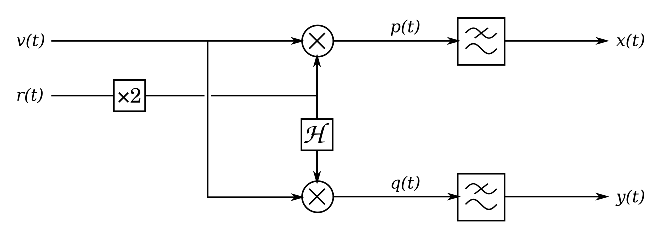
\includegraphics[width=\linewidth]{Images/lockin.eps}
	\caption{es un lockin}
	\label{fig:lockin}
\end{figure}


En la figura \ref{fig:lockin} hay un lockin

\section{Método Experimental}
En primer lugar se ensambló el circuito de la F1. sobre 
un protoboard. Con ésto se evaluó el funcionamiento del
lock-in en un circuito de carácter puramente resistivo 
en donde se pudo obtener el valor de la resistencia 
de carga RL.\\
Se utilizaron dos generadores de señal RIGOL DG4102 
para poder generar la señal de referencia y el ruido.
Para sumar éstas dos señales se tuvo que "flotar"[1] la 
tierra de uno de los generadores dado que éstos no poseen 
tierra propia, sino que utilizan la de la red eléctrica.\\

Para la realización del lock-in se implementó un 
script en python como se puede ver en el apéndice.
En el código se importó la librería del 
conversor analógico dígital USB-1408FS de la línea 
MEASUREMENT COMPUTING para poder 
calibrarlo y realizar las mediciones. Se implementaron 
las etapas de la \ref{fig:lockin}, en donde se optó 
por utilizar filtros FIR dada su versatilidad y sencillez.

\section{Resultados}

Se midió el valor de RL en función 
de la relación señal a ruido en la entrada para tres 
filtros FIR de distintos orden.
Se puede apreciar que el filto óptimo es el de mayor 
orden, dado que se utilizan mayor cantidad de 
mediciones para generar las señales medidas.

\begin{figure}[H]
	\centering
	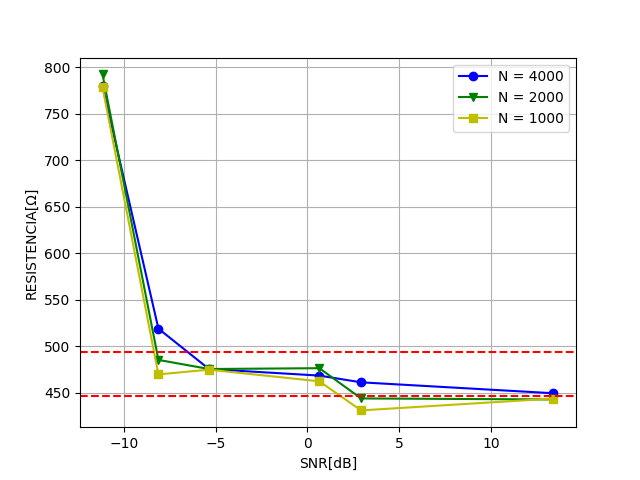
\includegraphics[width=\linewidth]{Images/RvsSNR(segunda).png}
	\caption{RvsSNR}
	\label{fig:RvsSNR}
\end{figure}

Para comprobar que el límite de funcionamiento 
del lock-in no está limitado por el orden del 
filtro elegido sino por la SNR a la entrada
se realizaron distintas mediciones 
sobre el valor RL(dada la simpleza del circuito) 
para un valor de SNR a la entrada de -22.5dB para 
distintos filtros como se explaya en la figura 
\ref{fig:RORDEN}. Se aprecia un valor mas acercado 
al tabulado cuando se aumenta el orden del filtro, sin 
embargo está lejos de entrar en la cota del error 
tabulado, y ésto afirma que el limitante en éste 
lock-in es el ruido a la entrada.\\

ESTARIA BUENO QUE EL ULTIMO PTO DE LA GRAFICA \ref{fig:RORDEN}
ESTE MAS ARRIBA PARA PODER HACER ESTA AFIRMACION 
VER SI CONVIENE PONER EN A TRABAJO FUTURO O MOVER EL PTO\\

\begin{figure}[H]
	\centering
	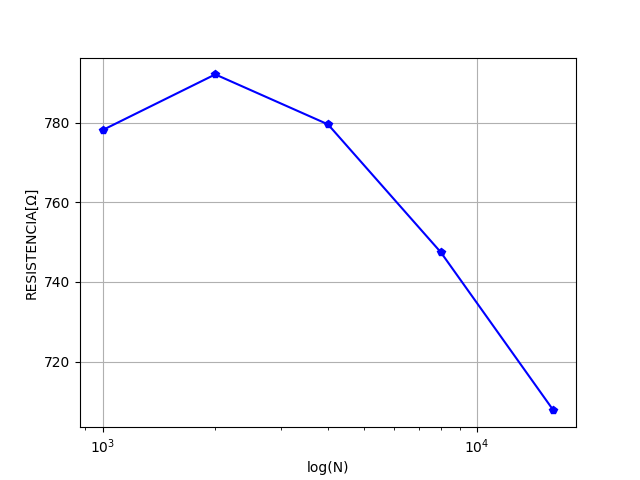
\includegraphics[width=\linewidth]{Images/RORDEN.png}
	\caption{RORDEN}
	\label{fig:RORDEN}
\end{figure}

Por último se armó el circutio de la F3. Con ésto 
se midió el valor de la capacidad CL para poder 
comprobar el funcionamiento del lock-in en 
impedancias complejas.

\begin{figure}[H]
	\centering
	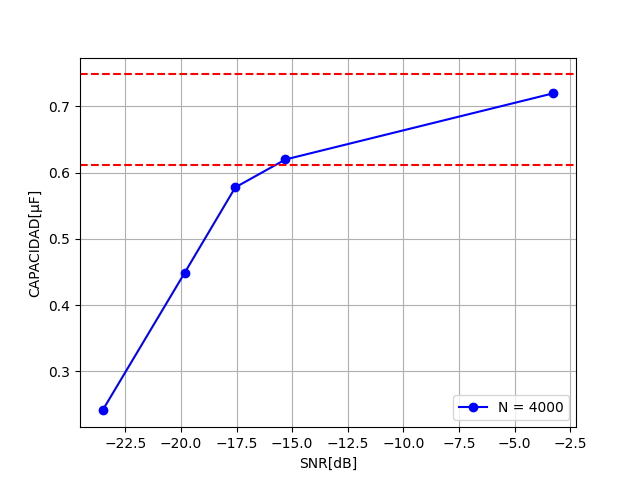
\includegraphics[width=\linewidth]{Images/CvsSNR(segunda).png}
	\caption{RvsSNR}
	\label{fig:CvsSNR}
\end{figure}


\section{Discusión}

\section{Conclusiones}



\bibliography{Antenas}
\bibliographystyle{ieeetr}

\end{multicols}
\newpage
\begin{appendices}
\vspace{-1em}
\hrule
\vspace{1em}
\normalsize
\section{Apéndice 1 - si pinta meter un apéndice}
\end{appendices}

\end{document}
